\chapter{Configure access and security for instances}
Openstack security groups are sets of IP filter rules that define
networking access and are applied to all instances within a project.
In the VSC cloud, each project contains a default security group,
which allows you to ping instances and connect using SSH.  You can add
rules to the default security group or add new security groups with
rules.

Key pairs are SSH credentials that can be automatically injected into
an instance when it is launched. To use key pair injection, the image
that the instance is based on must contain the \textbf{cloud-init}
package. Each project should have at least one key pair. For more
information, see the section \emph{Add a key pair} on page
\pageref{add-a-key-pair}.

\strong{Note:} In the VSC cloud, public keys you've uploaded to the
VSC account portal are automatically available in OpenStack projects.
Changes to your VSC account are reflected in the OpenStack environment
within 20 minutes.

If you have generated a key pair with an external tool, you can import
it into \gls{OpenStack}. The key pair can be used for multiple
instances that belong to a project. For more information, see the
section {\emph{Import a key pair}} on page
\pageref{import-a-key-pair}.  For general instructions on SSH keys, we
refer to chapter 2 of
\href{https://www.vscentrum.be/support/tut-book/vsc-tutorials}{the VSC
  HPC tutorial}.

\strong{Note:} A key pair belongs to an individual user, not to a
project. To share a key pair across multiple users, each user needs to
import that key pair.

\subsubsection{Add a key pair}\label{add-a-key-pair}
Create at least one key pair for each project.

\begin{enumerate}
\item Open the Compute tab.
\item Click the Key Pairs tab, which shows the key pairs that are
  available for this project.
\item Click Create Key Pair.
\item In the Create Key Pair dialog box, enter a name for your key
  pair, and click Create Key Pair.
\item Respond to the prompt to download the key pair.
  \end{enumerate}

\subsubsection{Import a key pair}\label{import-a-key-pair}

\begin{enumerate}
\item Open the Compute tab.
\item Click the Key Pairs tab, which shows the key pairs that are
  available for this project.
\item Click Import Key Pair.
\item In the Import Key Pair dialog box, enter the name of your key
  pair, copy the public key into the Public Key box, and then click
  Import Key Pair.
\item Save the \textbf{*.pem} file locally.
\item To change its permissions so that only you can read and write to
  the file, run the following command:

  \begin{prompt}
      %\shellcmd{chmod 0600 yourPrivateKey.pem}
  \end{prompt}

  \strong{Note:} If you are using the \gls{OpenStack Dashboard} from a
  Windows computer, use PuTTYgen to load the \textbf{*.pem} file and
  convert and save it as \textbf{*.ppk}.  For more information see the
  \href{https://winscp.net/eng/docs/ui_puttygen}{\emph{WinSCP web page
      for PuTTYgen}}, and chapter 2 of
  \href{https://www.vscentrum.be/support/tut-book/vsc-tutorials}{the
    VSC HPC tutorial}.

\item To make the key pair known to SSH, run the \textbf{ssh-add}
  command.

  \begin{prompt}
    %\shellcmd{ssh-add yourPrivateKey.pem}
  \end{prompt}
\end{enumerate}

The Compute database registers the public key of the key pair.

The \gls{OpenStack Dashboard} lists the key pair on the Key Pairs tab.

\subsubsection{Allocate a floating IP address to an instance}\label{allocate-a-floating-ip-address-to-an-instance}
When an instance is created in \gls{OpenStack}, it is automatically
assigned a fixed IP address in the network to which the instance is
assigned. This IP address is permanently associated with the instance
until the instance is terminated.

However, in addition to the fixed IP address, a floating IP address
can also be attached to an instance.  Unlike fixed IP addresses,
floating IP addresses can have their associations modified at any
time, regardless of the state of the instances involved.  In the VSC
cloud, floating IP's are public (accessible from the the Ugent login
node \lstinline{login.hpc.ugent.be}).  In order to make your instance
accessible from outside of the Openstack environment, you must attach
a port connected to the VM network to such a public floating IP.

This procedure details the reservation of a floating IP address from
an existing pool of addresses and the association of that address with
a specific instance.

\begin{enumerate}
\item Open the Network tab.
\item Click the Floating IPs tab, which shows the floating IP
  addresses allocated to instances.
\item Click Allocate IP To Project.
\item Choose the pool from which to pick the IP address.
\item Click Allocate IP.
\item In the Floating IPs list, click Associate.
\item In the Manage Floating IP Associations dialog box, choose the
  following options:

  \begin{itemize}
  \item The IP Address field is filled automatically, but you can add
    a new IP address by clicking the + button.
  \item In the Port to be associated field, select a port from the
    list.
  \end{itemize}

  The list shows all the instances with their fixed IP addresses.
\item Click Associate.
\end{enumerate}

Another way to associate a floating IP is after the user has already launched an instance which appears in the list of running instances in the Project-->Compute-->Instances tab:

\begin{enumerate}
\item Expand the drop-down menu on right next to the instance
\item Select Associate Floating IP
\begin{center}
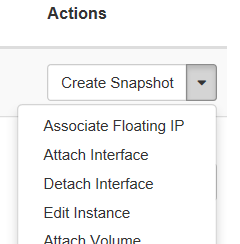
\includegraphics[scale=0.7]{img/associate_IP_1.png}
\end{center}
\item A pop-up window will appear and under IP Address select from the
  drop-down menu an IP address from the available pool.
\begin{center}
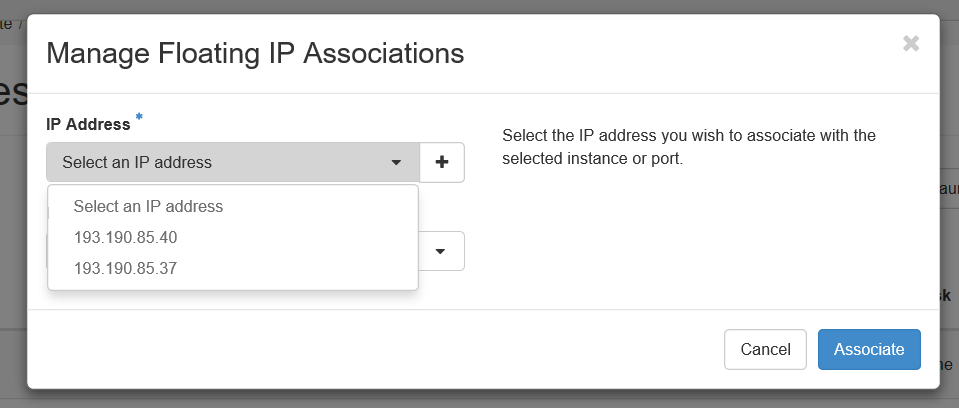
\includegraphics[scale=0.5]{img/associate_IP_2.png}
\end{center}
\item Click Associate
\end{enumerate}

If the IP has been successfully associated in the upper right corner of the browser screen will appear a green confirmation. If not successful a red notification will pop up that something went wrong.

\strong{Note:} To disassociate an IP address from an instance, click
the Disassociate button.  To release the floating IP address back into
the floating IP pool, click the Release Floating IP option in the
Actions column.

%%% Local Variables:
%%% mode: latex
%%% TeX-master: "intro-OpenStack"
%%% End:
